%iffalse
\let\negmedspace\undefined
\let\negthickspace\undefined
\documentclass[journal,12pt,twocolumn]{IEEEtran}
\usepackage{cite}
\usepackage{amsmath,amssymb,amsfonts}
\usepackage{graphicx}
\usepackage{textcomp}
\usepackage{xcolor}
\usepackage{txfonts}
\usepackage{listings}
\usepackage{enumitem}
\usepackage{mathtools}
\usepackage{gensymb}
\usepackage{comment}
\usepackage[breaklinks=true]{hyperref}
\usepackage{tkz-euclide} 
\usepackage{listings}
\usepackage{gvv}                                        
\def\inputGnumericTable{}                                 
\usepackage[latin1]{inputenc}                                
\usepackage{color}                                            
\usepackage{array}                                            
\usepackage{longtable}                                       
\usepackage{calc}                                             
\usepackage{multirow}                                         
\usepackage{hhline}                                           
\usepackage{ifthen}                                           
\usepackage{lscape}
\usepackage[export]{adjustbox}
\newtheorem{theorem}{Theorem}[section]
\newtheorem{problem}{Problem}
\newtheorem{proposition}{Proposition}[section]
\newtheorem{lemma}{Lemma}[section]
\newtheorem{corollary}[theorem]{Corollary}
\newtheorem{example}{Example}[section]
\newtheorem{definition}[problem]{Definition}
\newcommand{\BEQA}{\begin{eqnarray}}
	\newcommand{\EEQA}{\end{eqnarray}}
\newcommand{\define}{\stackrel{\triangle}{=}}
\newtheorem{rem}{Remark}

\begin{document}
	\parindent 0px
	\bibliographystyle{IEEEtran}
	
	\vspace{3cm}
	
	\title{}
	\author{EE23BTECH11209 - K S Ballvardhan$^{*}$
	}
	\maketitle
	\newpage
	\bigskip
	
	% \renewcommand{\thefigure}{\theenumi}
	% \renewcommand{\thetable}{\theenumi}
	
	
	
	
	\textbf{Question:} A series of natural numbers F$_1$, F$_2$, F$_3$, F$_4$, F$_5$, F$_6$, F$_7$,....obeys F$_{n+1}$ = F$_n$ + F$_{n-1}$ for all integers n $\geq$ 2.
	If F$_6$ = 37, and F$_7$ = 60, then what is F$_1$? \hfill[GATE CS 2023]
	
	\textbf{Solution: }
	
	\begin{table}[ht] 
		\centering
		\begin{tabular}{|c|c|c|}
    \hline
    \textbf{Parameter} & \textbf{Description} & \textbf{Value} \\
    \hline
    $ x\brak 6$ & Seventh term of the sequence & 60 \\
    \hline
    $ x\brak 5$ & Sixth term of the sequence & 37 \\
    \hline
    $ x\brak 1$ & Second term of the sequence & ? \\
    \hline
    $ x\brak 0$ & First term of the sequence & ? \\
    \hline
    \end{tabular}


		\caption{input values}
		\label{tab: Table2022cs36}
	\end{table}
	
	Let the sequence be:
	\begin{align}
	1, F_2, F_3 \dots
	\end{align}
	Given recurrence relation is
	\begin{align}
	F_{n+1} &= F_n + F_{n-1}
	\end{align}
    Taking z-transform of $ F_n$:
	\begin{align}
		F\brak{z} &= F_1 + z^{-1} F_2 + \sum_{n=2}^{\infty} F_n z^{-n}\\
	    &= F_1 + z^{-1} F_2 + z^{-1} \sum_{n=1}^{\infty} F_{n+1} z^{-n}\\
	    &= F_1 + z^{-1} F_2 + z^{-1} \sum_{n=1}^{\infty} \brak{F_n + F_{n-1}}z^{-n}\\
	    &= F_1 + z^{-1} F_2 + z^{-1}\brak{F\brak{z}-F_1 + z^{-1}F\brak{z}}\\
		\implies F\brak{z}&= \frac{F_1 + \brak{F_2-F_1}z^{-1}}{1-z^{-1}-z^{-2}}
	\end{align}
	Using Contour Integration to find the inverse $Z$-transform,
	\begin{align}
		F_{n}&=\frac{1}{2\pi j}\oint_{C} F\brak{z} \;z^{n-1} \;dz  \\
		&=\frac{1}{2\pi j}\oint_{C}\frac{z^{n}\brak{F_2-F_1+F_1 z}}{z^2-z-1} \;dz 
	\end{align}
	
	By residue theorem:
	
	\newpage
	
	\begin{align}
		\notag F_n&=\frac{1}{\brak {0}!}\lim\limits_{z\to {\frac{1+\sqrt{5}}{2}}}\frac{d}{dz}\brak {{(z+\frac{1+\sqrt{5}}{2})}F\brak{z}}\\ &+ \frac{1}{\brak {0}!}\lim\limits_{z\to \frac{1-\sqrt{5}}{2}}\frac{d}{dz}\brak {{\brak{z+\frac{1-\sqrt{5}}{2}}}F\brak{z}}
	\end{align}
	On simplifying we get,
	\begin{align}
		\notag F_n &= \brak{F_2-F_1}\brak{\brak{\frac{1+\sqrt{5}}{2}}^n-\brak{\frac{1-\sqrt{5}}{2}}^n}\\ &+ \brak{F_1}\brak{\brak{\frac{1+\sqrt{5}}{2}}^{n+1}-\brak{\frac{1-\sqrt{5}}{2}}^{n+1}}
	\end{align}
	From the values in \tabref{tab: Table2022cs36}:
	\begin{align}
		5 \brak{F_2-F_1} + 8 F_1 &=37\\
		8 \brak{F_2-F_1} + 13 F_1 &=60\\
		\implies F_2 =5, F_1 &=4
	\end{align}
	\begin{align}
		\therefore \boxed{F_1=4}
	\end{align}
	\begin{figure}[ht]
		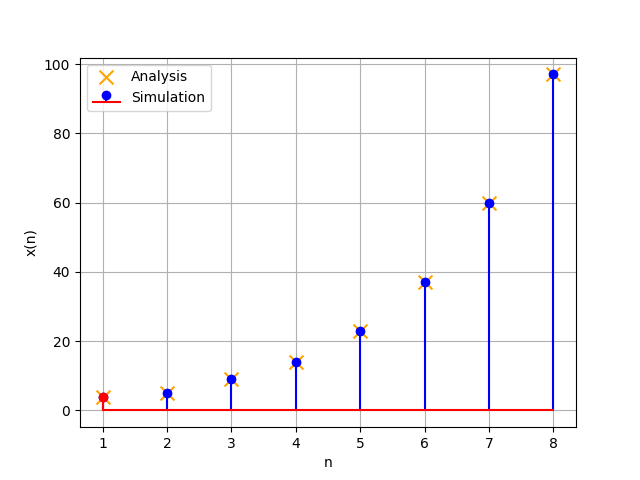
\includegraphics[width = \columnwidth]{figs/fig4}
		\caption{Terms of the given sequence}
		\centering
		\label{fig: fig4}
	\end{figure}
	
\end{document}
